\documentclass[12pt]{article}
\usepackage{amsmath,amssymb,amsthm}
\usepackage[english]{babel}
\usepackage[utf8]{inputenc}
\usepackage{fancyhdr}
\usepackage{changepage} 

% for line spacing
\usepackage{setspace}

% for absolute value
\usepackage{commath}

% for numbering
\usepackage{enumerate}

% for image placing
\usepackage{float}

% paper size and margins
\usepackage[letterpaper, left=20mm, right=20mm, top=25mm, bottom = 25mm, headsep=.15in]{geometry}

% for curly brace
\usepackage{amsmath}

% for input images
\usepackage{graphicx}
\graphicspath{ {./} }

% for printing pseudocode
\usepackage[boxed]{algorithm}
\usepackage[noend]{algpseudocode}

% for tables
\usepackage{tabularx}

\makeatletter
\def\BState{\State\hskip-\ALG@thistlm}
\makeatother

% for circled numbers
\usepackage{tikz}
\newcommand*\circled[1]{\tikz[baseline=(char.base)]{
            \node[shape=circle,draw,inner sep=1pt] (char) {#1};}}

% double line space
\renewcommand{\baselinestretch}{2.0}

% header, footer and page number
\pagestyle{fancy}
\fancyhf{}
\rhead{Tiankai Jiang \quad 20834939}
\lhead{ECE657A \quad Assignment 1}
\fancyfoot[C]{\thepage}

\setlength{\headheight}{15pt}

\begin{document}
\noindent
1.
\begin{center}
    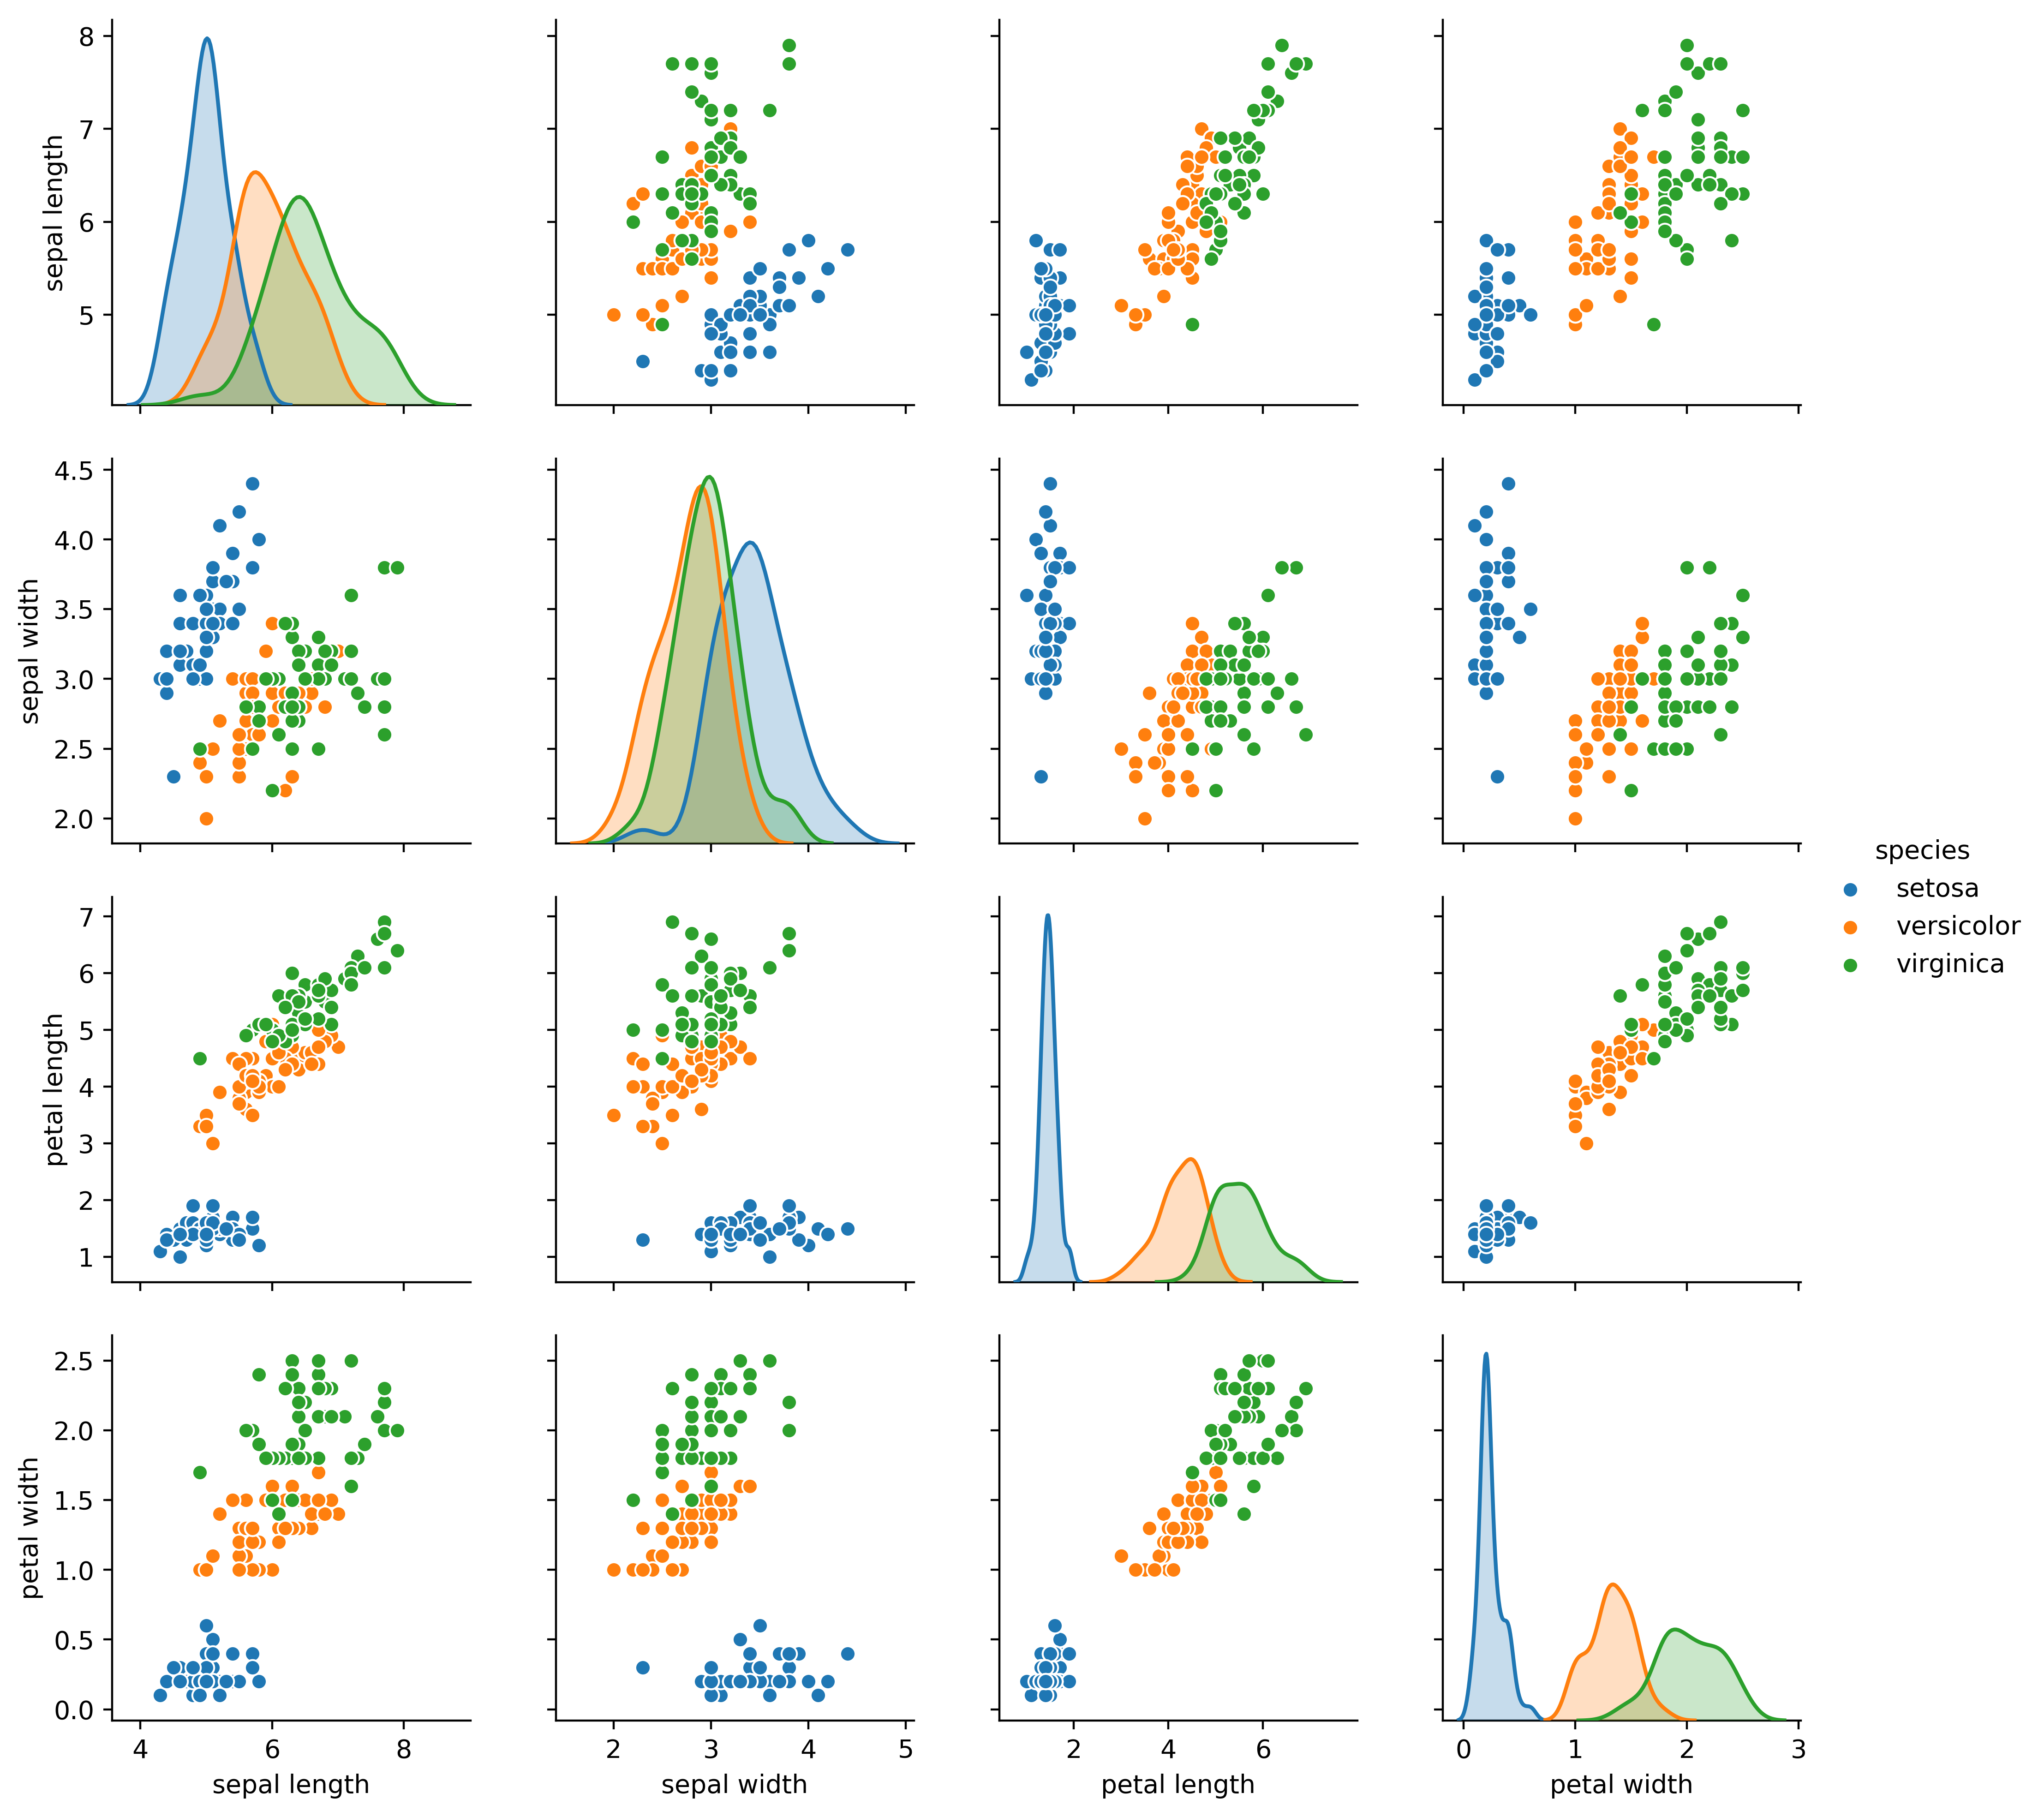
\includegraphics[width=17cm]{Q1.png}
\end{center}
Setosa is the most distinguishable species among the three, as it has the smallest petal width and petal length. Basically all points are distributed on the plot with petal length $\leq$ 2cm and petal width $\leq$ 1cm.\\
With the same sepal length or sepal width or petal length, versicolor tends to have a smaller petal width and petal length than virginica. But there is no clear boundary between them and the distribution of their points are not as dense as setosa's. Also, it is extremely difficult to separate versicolor and virginica based on sepal width.\\
Regardless of flower species, there is a strong, positive, linear relationship between petal length and petal width. And there is a moderately strong, positive, linear relationship between sepal length and petal length, sepal length and petal width. However, there is no such relationship between sepal width and other features.
\newpage
\noindent
2.\\
Accuracy with default k is $96.67\%$.
\begin{center}
    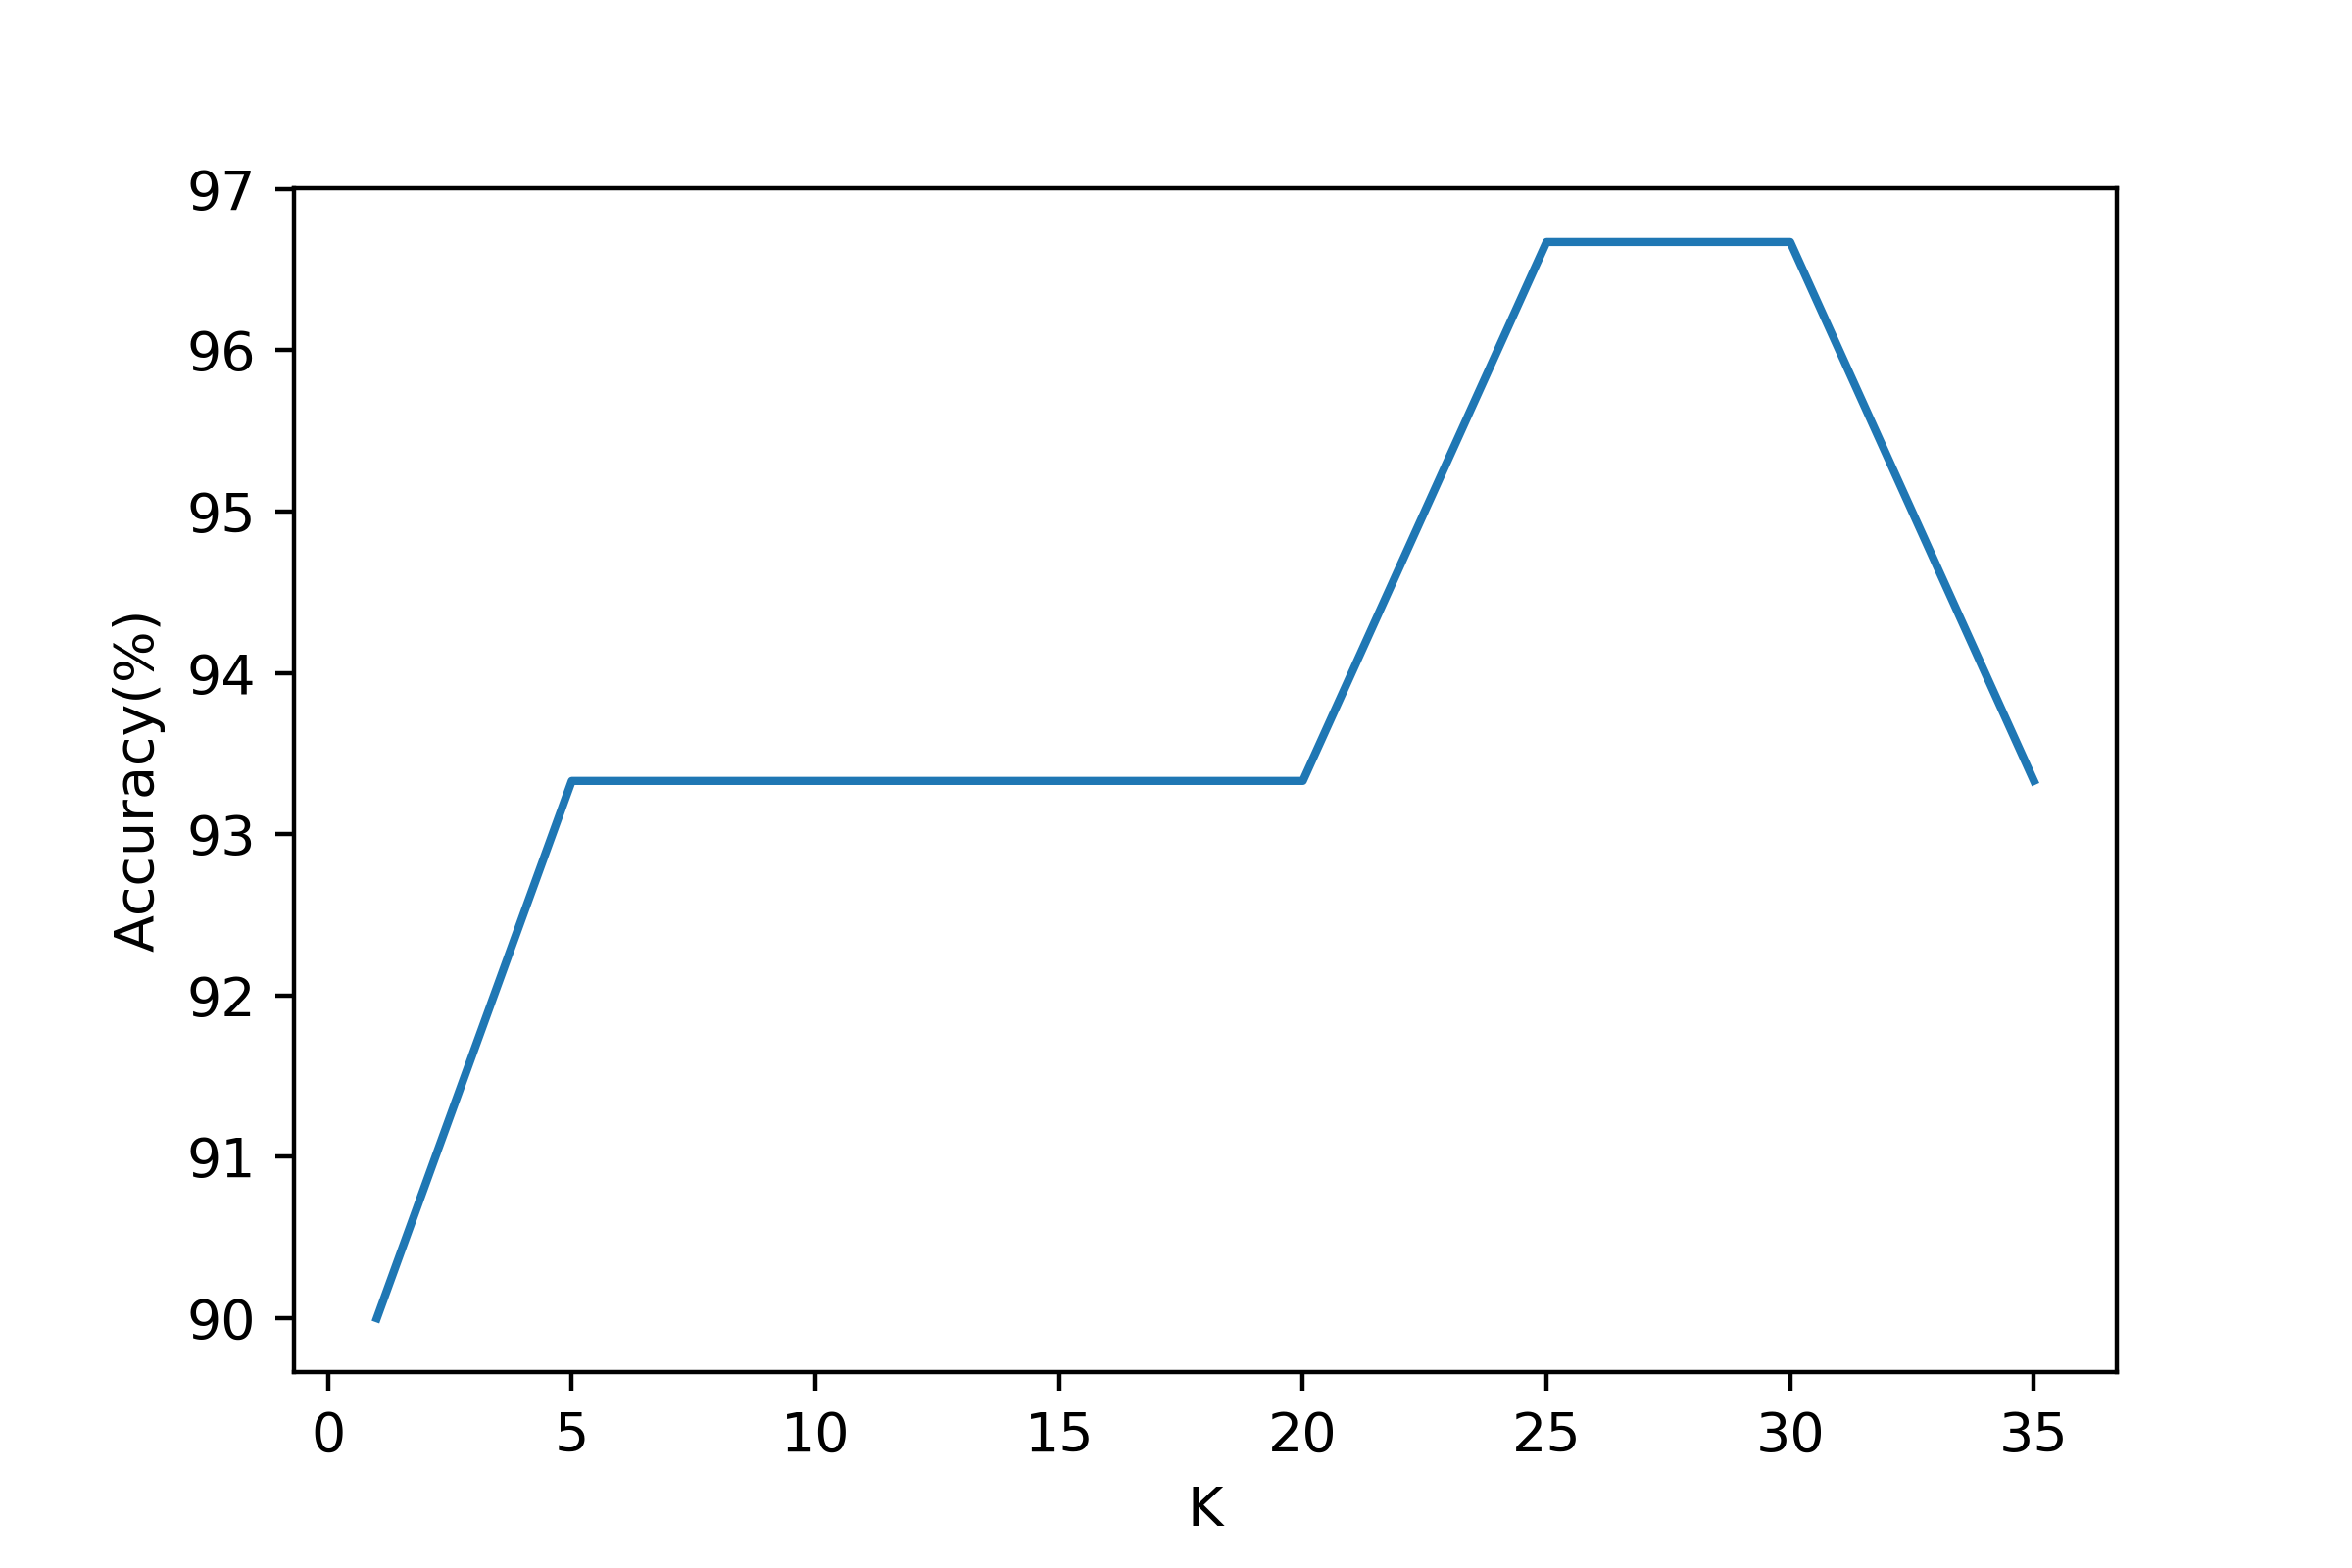
\includegraphics[width=10cm]{Q2.png}
\end{center}
The best parameter for KNN is 25. Checking 25 nearest neighbours is more efficient than checking 30 of them. The accuracy on test set is $100.00\%$.
\newpage
\noindent
3.
\begin{center}
    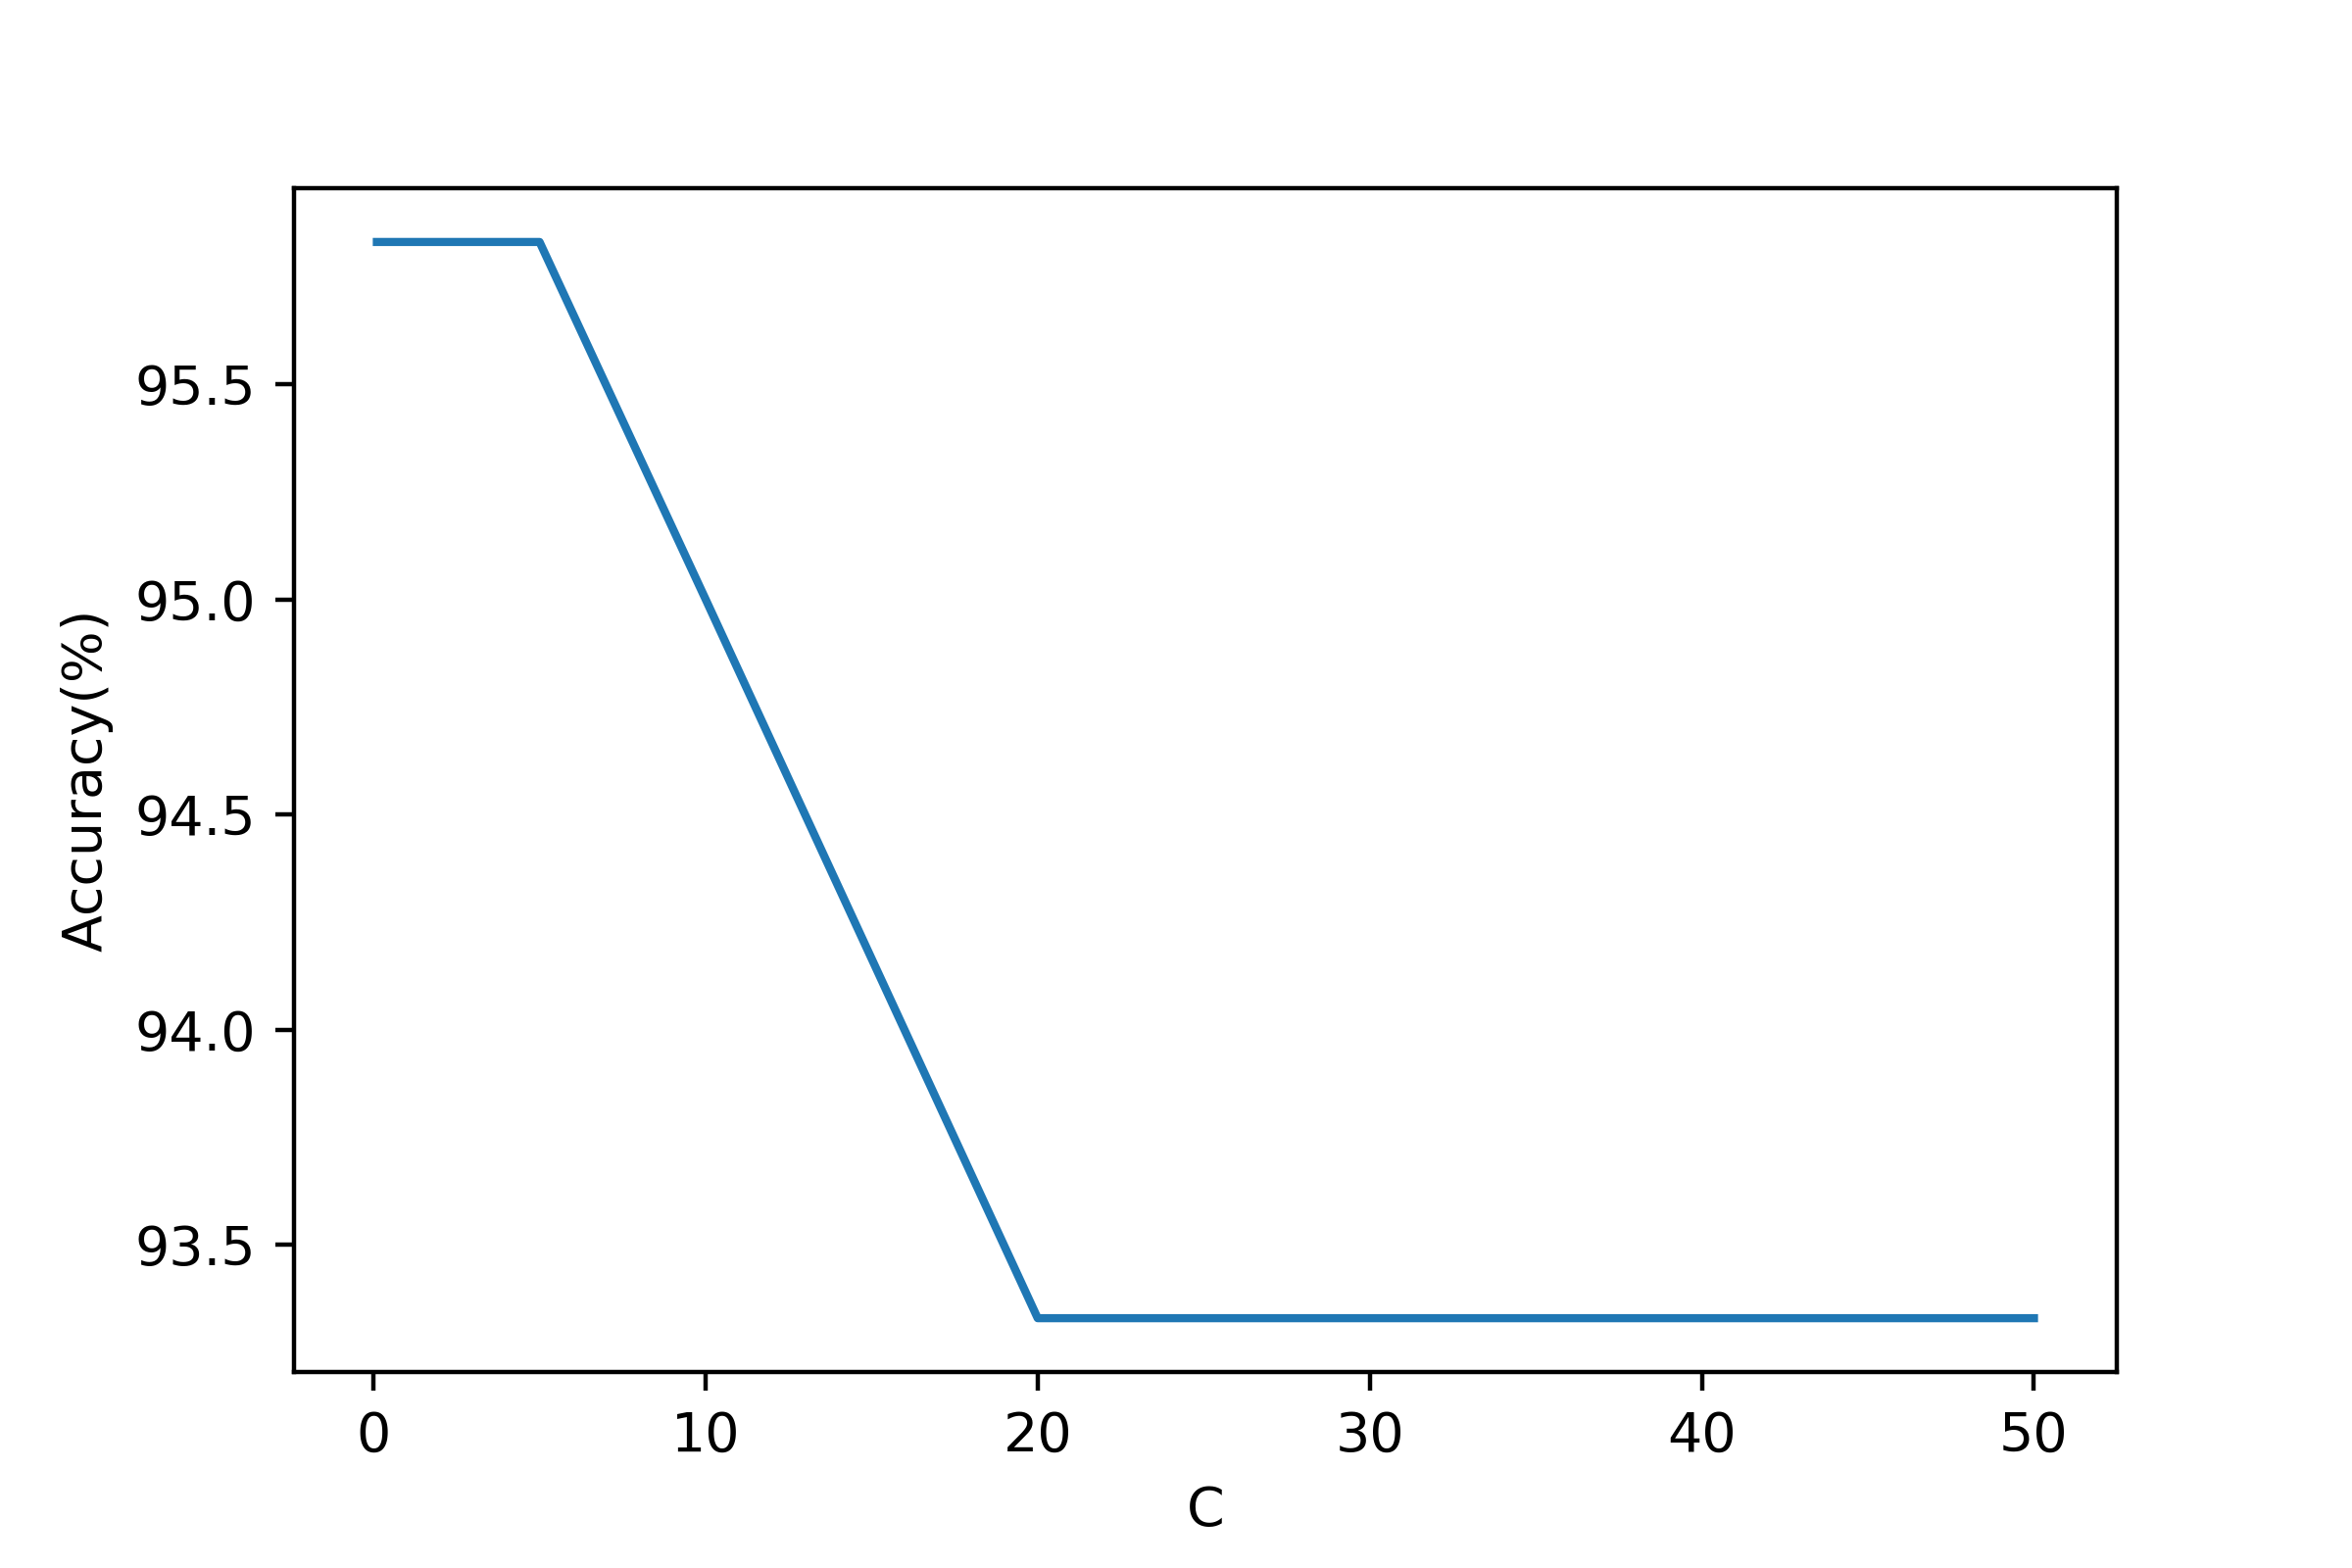
\includegraphics[width=10cm]{Q3.png}
\end{center}
The best parameter for SVM is $C=1$. $C=0.1,0.5,1,2,5$ all gave the highest accuracy. But $C=1$ is in the middle of them therefore the model with $C=1$ will have a moderate margin and fault tolerance among these parameters. The accuracy on test set using $C=1$ is $100.00\%$.
\newpage
\noindent
4.
\begin{center}
    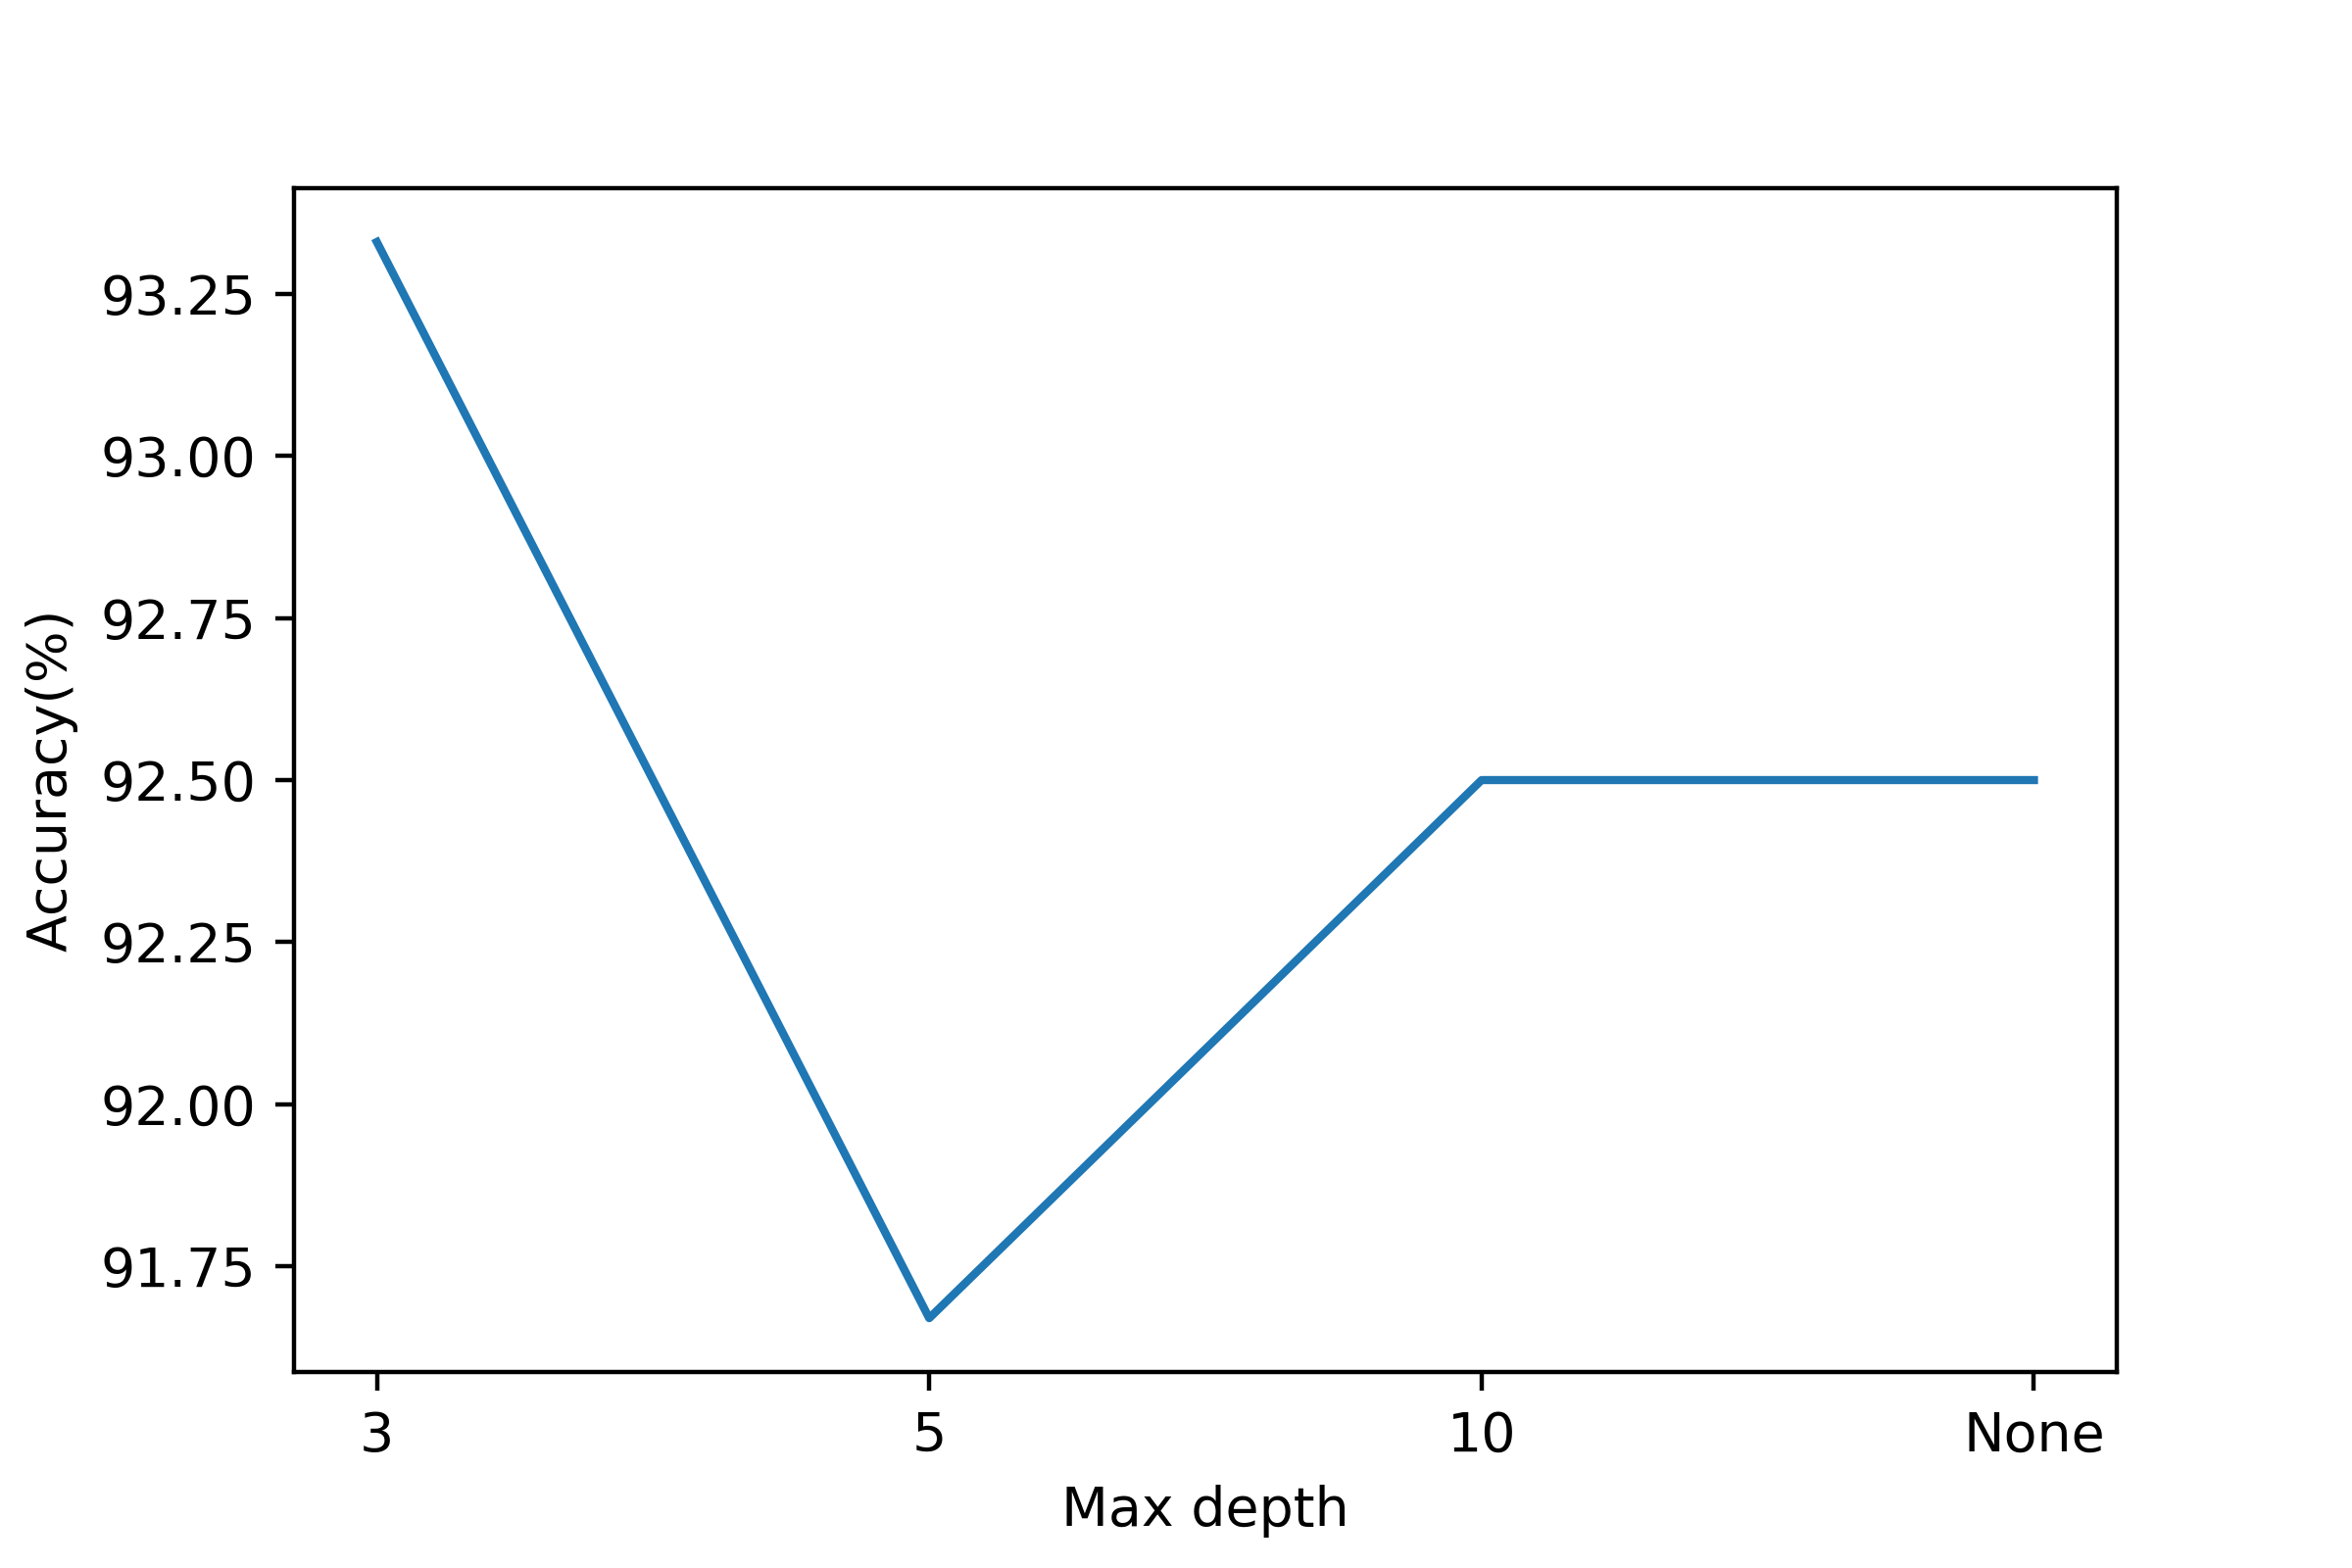
\includegraphics[width=10cm]{Q4a.png}
\end{center}
The best parameter for decision tree is max depth = 3. The accuracy on test set using $max-depth=3$ is $100.00\%$.
\begin{center}
    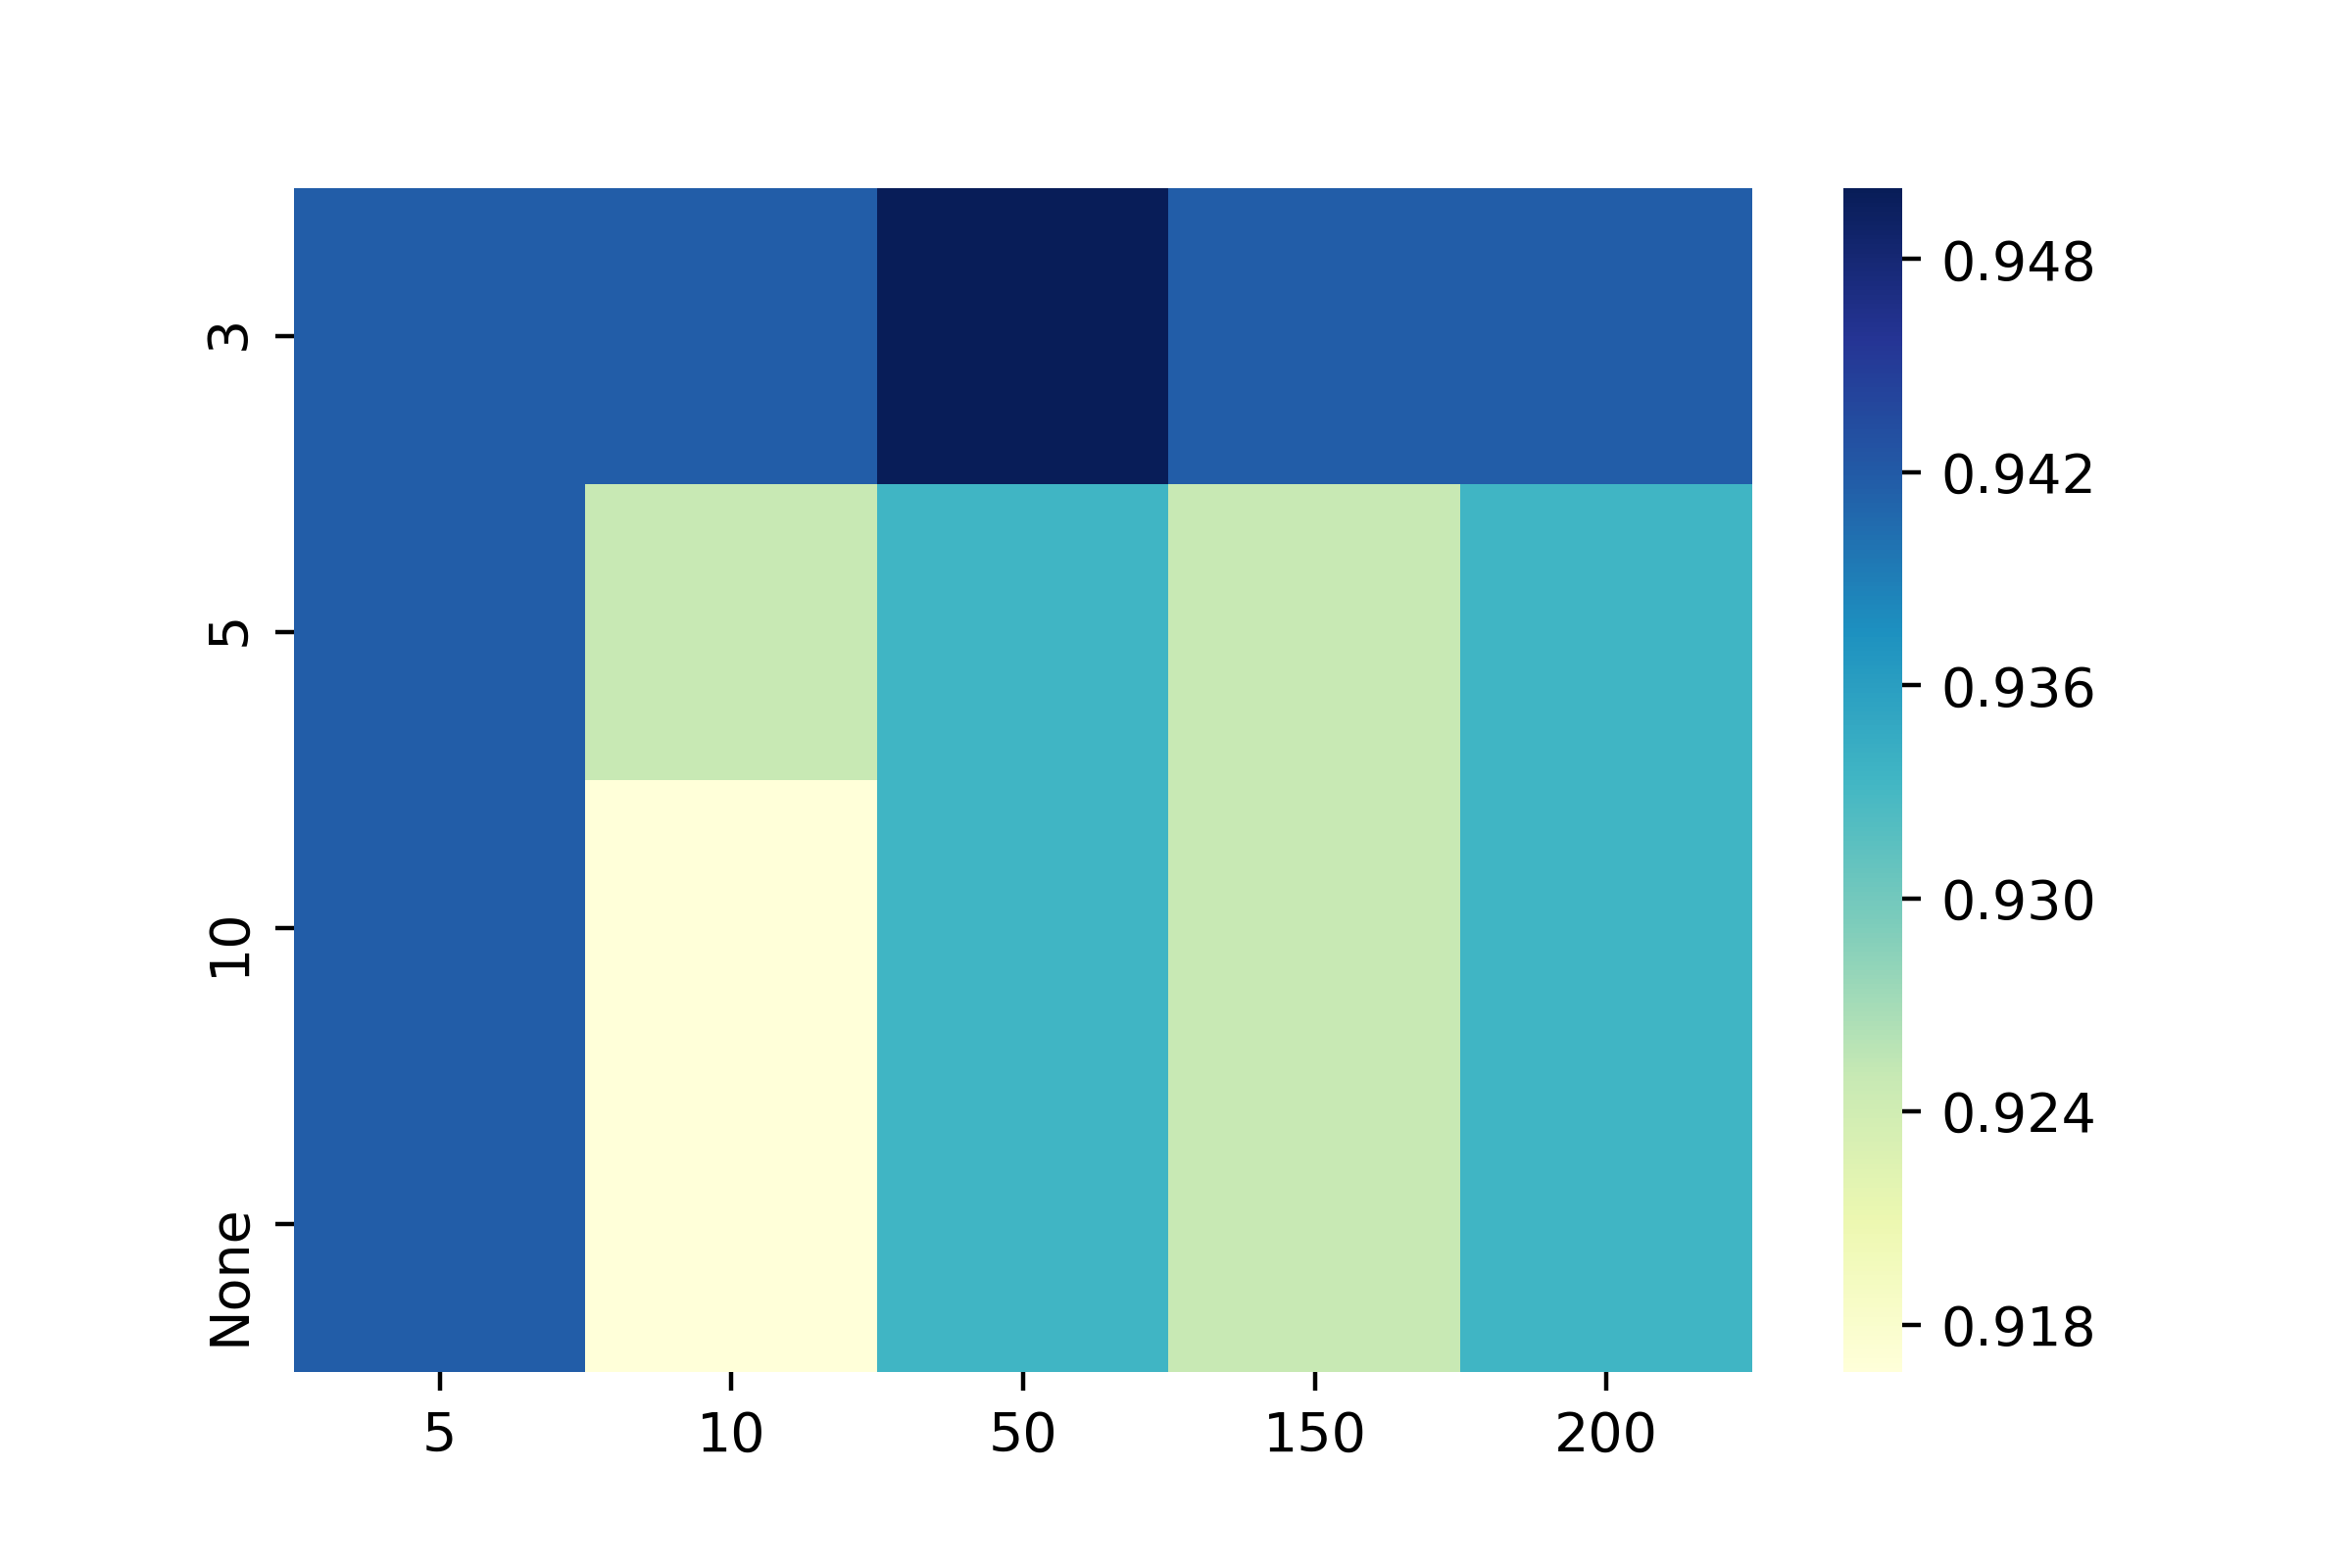
\includegraphics[width=10cm]{Q4b.png}
\end{center}
The best parameter for random forest is max depth = 3 and n estimator = 50. The accuracy on test set using $max-depth=3$ and $n-estimator=50$ is $100.00\%$.
\begin{center}
    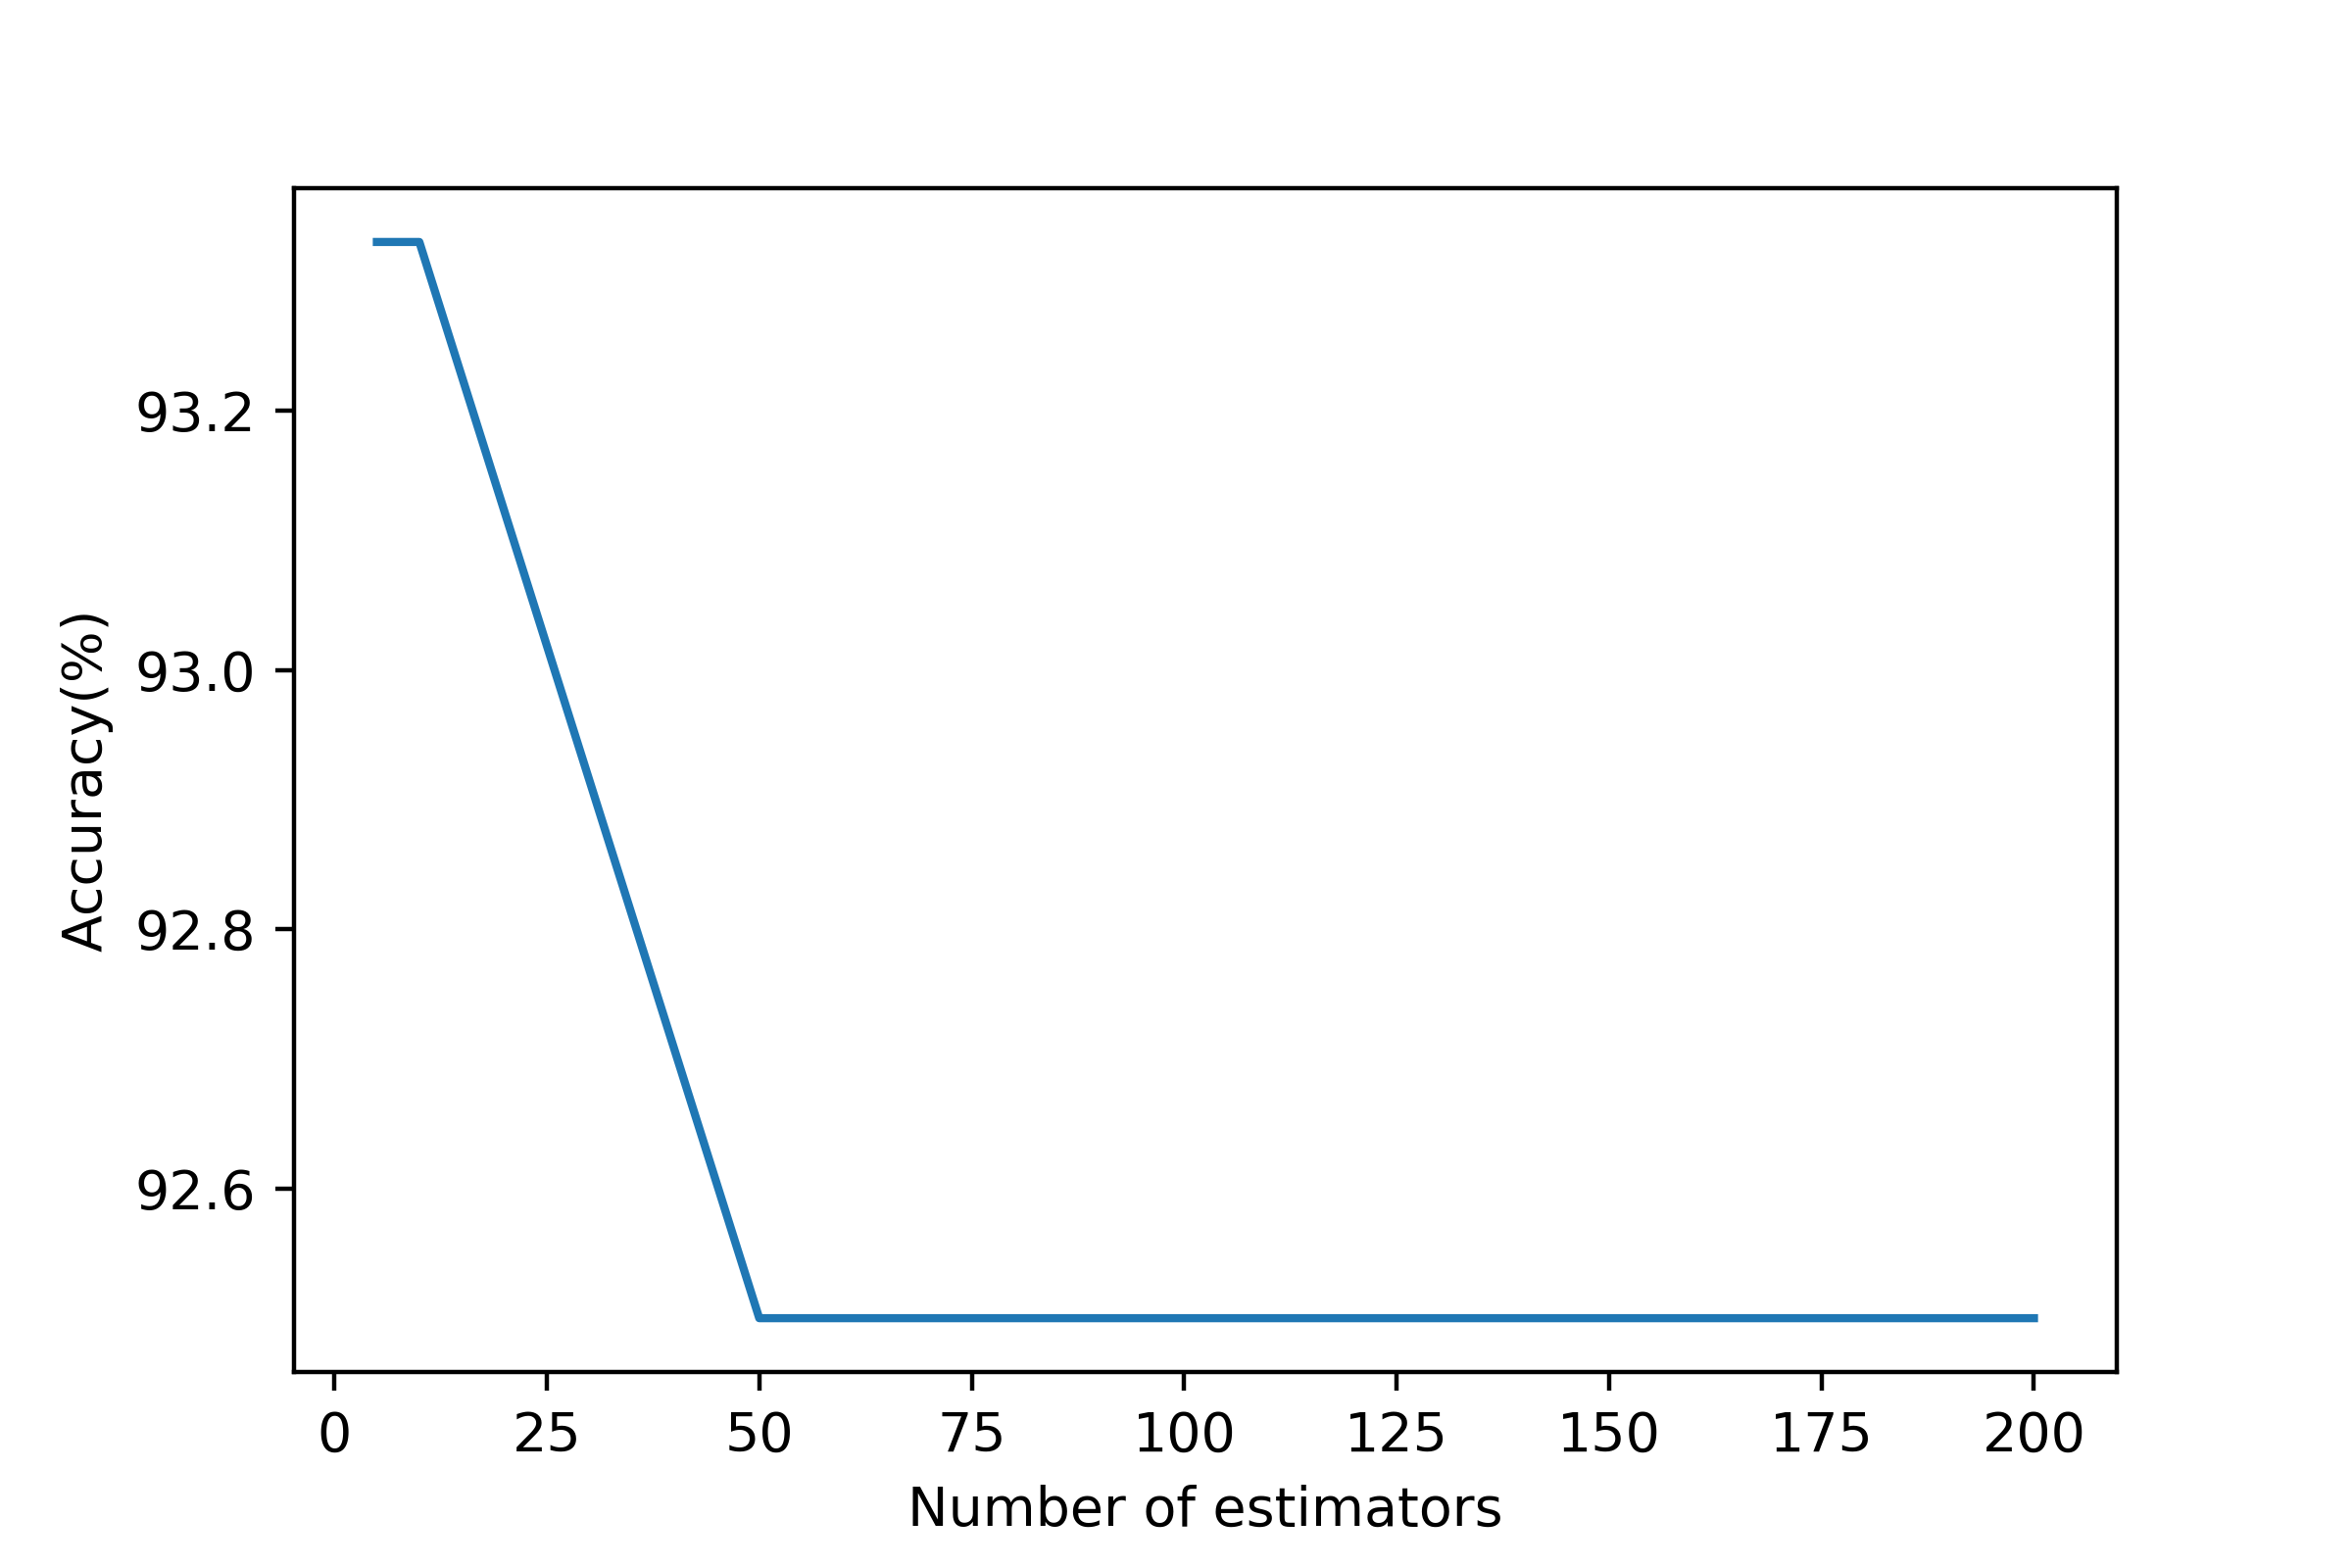
\includegraphics[width=10cm]{Q4c.png}
\end{center}
The best parameter for gradient boost is n-estimator = 5. Although n-estimator=10 gives the same result, it uses unnecessary trees and decreases efficiency. The accuracy on test set using $n-estimator=50$ is $100.00\%$.
\newpage
\noindent
5.
\begin{enumerate}[i)]
  \item Explain why you had to split the dataset into train and test sets? \\
  We want to test the model to make sure it performs well on all datasets. We cannot use the training data again since a good result means nothing, or a potentially overfit model. Using the test set, which is never presented to the model before, we can make a fair evaluation on our model. 
  \item Explain why when finding the best parameters for KNN you didn’t evaluate directly on the test set and had to use a validation test.\\
  To find the best parameters, the variables are the parameters. According to control variates method, each time there should only be one variable. Hence, the test set should not change. If we evaluate directly on the test set, we have to find another dataset to test the model, which introduces another variable, which is against the control variates method.
  \item What was the effect of changing k for KNN. Was the accuracy always affected the same way with an increase of k? Why do you think this happened?\\
  Changing k changes the accuracy of a model. The accuracy was not always affected the same way with an increasing k. When k is too small, the model may be overfit since the noise affect the decision process. When k is too large, the model may be underfit since a lot of data from other classes may affect the decision process. Hence, the accuracy is likely to increase first then decrease as k increases from 1.
  \item What was the relative effect of changing the max depths for decision tree, random forests, and gradient boosting? Explain the reason for this.\\
  As the max depth increases, the training error will always be non-increasing. However, the testing error will decrease first and start to increase at some point, since a tree with low max-depth cannot reflect the pattern in datasets and a tree with high max-depth will overfit the training data. The best max-depth lies somewhere between them.
  \item Comment on the effect of the number of estimators for Gradient Tree Boosting and what was the relative effect performance of gradient boosting compared with random forest. Explain the reason for this.\\
  In general, the more trees we use, the better the result. But as we add more trees, the improvement on the accuracy decreases and the computational cost inceases. At some point, the improvement becomes so little that it is not worth adding more trees. As the number of trees increases, the result of gradient boosting improves mainly because the bias is reduced, for gradient boosting uses weak learners(shadow trees). On the other hand, the result of random forest improves mainly because the variance is reduced, for random forest uses fully grown trees.
  \item What does the parameter C define in the SVM classifier? What effect did you observe and why do you think this happened?\\
  C is the penalty parameter of the error term in linear SVM objective function: $\frac{1}{2}w^Tw+C\sum\limits_{i=1}^{l}\xi_i$ A smaller C allows more misclassification and creates a larger margin when training SVM, and a larger C allows less misclassification and a smaller margin hyperplane on the training set.
\end{enumerate}
\end{document}